% !TEX root=frame_thesis.tex
\chapter{Methods and Model Description}

\section{Overview of the Model}
%Topic: General overview of ABM
%Main Idea: Human agents interact with local Environment
In this thesis, I present an Agent Based Model (ABM) that simulates the temporal and spatial pattens of household agents on Easter Island and their interaction with the natural environment. 
The environment is encoded on a 2D discretised map with real geographic features.
Agents rely both on a non- or slowly renewable resource, the palm trees, and a renewable resource, land for agriculture, in particular sweet potato cultivation. 
They obtain these resources by cutting trees and occupying viable sites with gardens in their near surroundings, thereby changing their local environment.
Consequently, the household's population growth or decline depends on the success of this resource allocation. 
Furthermore, resource availability determines the settlement behaviour of the agents.
The interaction with the natural environment places constraints on the settlement patterns as well as the population dynamics of the overall Easter Island society.

%Topic: Time and Update Order
The model assumes yearly updates of the variables of each household agent and the environment throughout the time period of the prehistoric Easter Island society.
The simulation starts with the arrival of the first settlers at Anakena Beach in $t_\text{arrival} = 800\, {\rm A.D.}$. 
The initial population is assumed to be 40 individuals spread on 2 households (40 in \citet{Good2006} and 20 to 100 in \citet{Brander1998}, 50 in \citet{Brandt2015}).
In each time step, $\Delta t=1\,{\rm yr}$, all agents are updated sequentially in a random order. 
A single update comprises the interaction between the agent and the environment, consequent changes of the variables, adjustment of the agent specific parameters, population growth/decline and potential re-settlement.
New household agents can appear throughout the simulation following reproduction and splitting of existing agents. 
The simulation ends in $1800\, {\rm A.D.}$ with the arrival of European voyages marking the end of the isolated status of the Easter Island society.%, since this presumably had a large impact on the society, e.g.\ through the introduction of diseases wiping out a large fraction of the Easter Island population in the 19th century.% \todo{cite Bahn2017}.

%Topic: I will describe the Model
In Section \ref{sec:CreateMap}, I describe the generation of the 2D discretised map comprising the environment of Easter Island. In Section \ref{sec:AgentUpdate}, I then focus on the household agents and the update of a single agent.
This update is separated into several modules: Calculating of the agents' resource requirements, cutting trees, farming, increasing/decreasing population of the agent, and potentially moving the settlement.
Figure \ref{fig:SketchABM} summarises all environmental variables, the agent variables, and their dependencies.


\begin{figure}[H]
	\centering
	%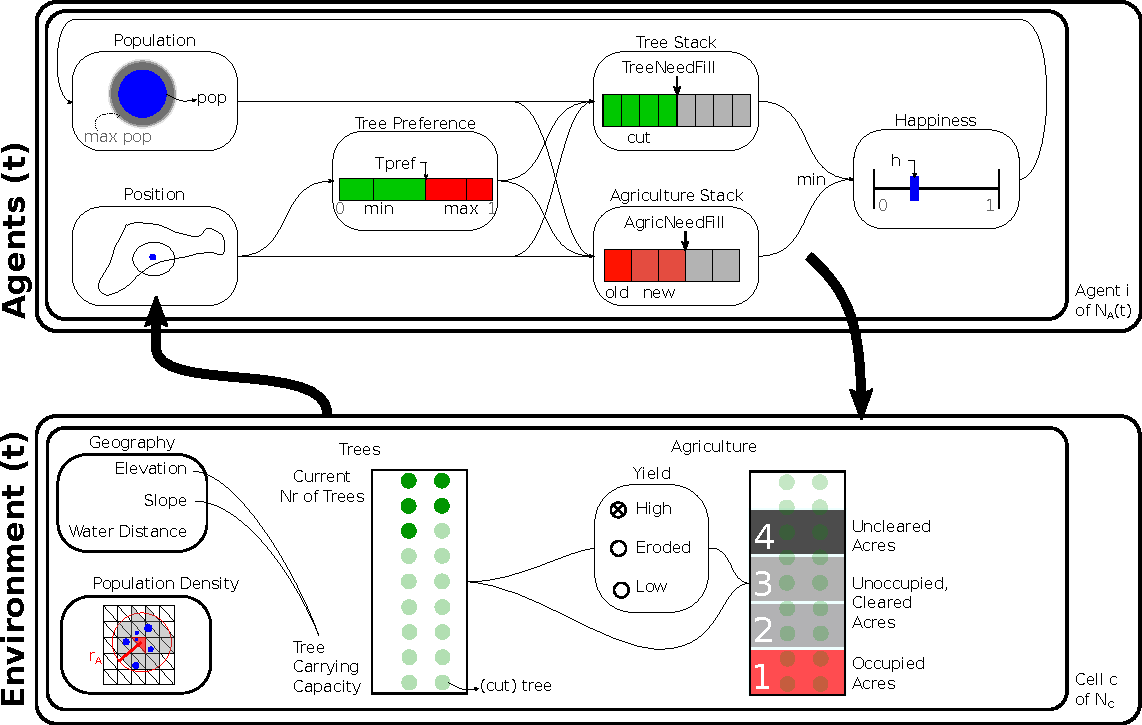
\includegraphics[width=1\textwidth]{images/SketchABM/SketchABM.pdf}
	\caption{
		A sketch of the ABM presented here and described in detail in Chapter \ref{chapter:Methods}.
		The environment consists of $N_\text{c}$ discretised cells, $c$, with certain geographic properties: Terrain elevation $el(c)$, slope $sl(c)$, area, $A(c)$, %population density $\frac{pop(C_\text{F}(t)}{r_\text{F}^2\pi}$) (within cells in a circle with radius $r_F$, $C_F(c)$) 
		and the two `resource stock' variables.
		The first stock variable of a cell is the number of trees $T(c,t)$.
		The maximum stock is the cell's carrying capacity and initial state, $T(c,t=0)$, which depends on the terrain elevation $el(c)$ and $sl(c)$. 
		The second stock of a cell is the number of arable (i.e.\ Productivity index $F_{\rm PI}(c,t)>0$) sites, $F_\text{arable}(c,t)$, with a basic unit of $1\, {\rm acre}$, in combination with the number of occupied sites, $F_\text{occ}(c,t)$ in acres.
		Agents are households with a population size $pop_\text{i}(t)$, a settlement location $(x_\text{i},\, y_\text{i})$ (corresponding cell $c_\text{i}(t)$), a tree preference $T_\text{pref, \, i}(t)$ depending on the tree stock of the local environment, and corresponding requirements for tree cutting, $T_\text{req, \, i}(t)$ and farming, $F_\text{requ, \, i}(t)$, depending on the tree preference and global constants, baseline tree and farming requirements per person, $T_{requ, \, pP}$ and  $F_\text{requ, \, pP}$.
		The success of meeting these requirements depends on the resource stocks of cells in radii $r_T$ for tree harvest and $r_F$ for farming. 
		The resulting current and smoothed happiness indices, $h_\text{i}(t)$ and $H_\text{i}(t)$ then determine the agent's population dynamics.
		Finally, for insufficiently small smoothed happiness (i.e.\ when the agent's net population size decreases) the settlement is moved to a new location in a complex, semi-rational, individual decision making process through evaluating sites according to multiple environmental factors.
	}
	\label{fig:SketchABM}
\end{figure}


\section{Creating a 2D discretised Map of Easter Island}

First, a discretised map is created dividing the island into a number of small 2D triangular cells with certain geographical features via a triangulation of a rectangular grid of points.
I use a 2D equidistant grid ranging from $(-27.2050^\circ N, \, -109.4650^\circ E)$ to $(-27.0437^\circ N, \, -109.2227^\circ E)$ and a resolution of \todo{$points/km^2$}(i.e.\ $100$ points in $x$(East)- and $50$ points in $y$(North)-direction).. 
In principle, the map can be created with any arbitrary resolution, constrained only by the resolution of the underlying geographical data. 
Also other grid types, e.g.\ one with higher resolution in a specific region of interest, are completely compatible with the model. 
While a higher resolution results in a more detailed and less discretisation error, computation time of the presented model scales highly non-linearly (see Section \TODO).
Hence, a trade-off has to be found between detail or accuracy and computation time.
Given this grid, I use \citet{matplotlib}\TODO's Delaunay triangulation tool to create 2D triangular cells.
A cell's location is defined by its midpoint $\vec{c} = (c_x,\, c_y)$. 
Since all cells are Delaunay triangles, the smallest angle is maximised. 
Hence, the midpoint, $\vec{c}$, provides a reasonable representation of the cell.
%Topic: Define Easter Island
%Using geographical information, the triangles making up Easter Island are selected.
The terrain features, elevation, $el(c)$, and slope, $sl(c)$, of Easter Island are obtained from a publicly available, high resolution elevation map \citep{Jarvis2008CIGAR} via Google Earth Engine \citep{gorelick2017google} and evaluated at the midpoint $\vec{c}$.
All cells located on the ocean (i.e.\ $el(c)=0$) are masked out and discarded.
The remaining ones constitute the landmass of the discretised island. 
With the resolution given above, $N_c = 11387$ cells remain. 
The area of the discretised Easter Island is $A=\TODO$, i.e.\ only a negligible fraction off from the $163.6\, {km^2}$ in reality.
with a area of once cell of $\overline{A(c)}= todo \pm todo$ \TODO.  
There are three -- or two in periods of major droughts (see \citet{Rull2020}) -- permanent crater lakes on Easter Island, providing the major freshwater sources for the prehistoric Easter Island population, as discussed later in Section \ref{sec:Moving}.
The corresponding cells are calculated from the locations and radii of these lakes. 
This procedure gives a detailed, discretised representation via triangular cells with geographical features of Easter Island. 
 
%Archaeological records indicate that crater lakes could have dried out during major drought periods.
%In particular the drying of Rano Raraku in the East of Easter Island during the Medieval Climate Anomaly ($500-1200 \, \rm{A.D.}$) and during the Little Ice Age ($1570-1720\, \rm{A.D.}$) \citep{Rull2020} and the consequences have been a reoccuring theme of scientific debate (e.g.\ \citet{Cauwe2011}). 
%Such drought events can be simulated by removing each of the lakes for some period of time from the map.

Furthermore, all cells have constant biological features.% next to the geographic specification before. 
Each cell $c$ has a variable tree number, denoted as $T(c,t)$ (or tree density $T(c,t)/A(c)$.
At the time of the arrival of the first settlers, the islands forest system was in equilibrium (e.g.\ \citet{Brander1998}) except for possible climatic changes, which impacted tree cover change over time \citep{Rull2020}, which are not considered here. 
Therefore, the tree number on each cell before human occupation $T(c,t=t_\text{arrival})$, constitutes a carrying capacity of palm trees for this cell. 
I assume this carrying capacity to be constant throughout the simulation.
There is is still a lot of uncertainty about the total number and patterns of palm trees at the time of arrival of the first settlers. 
\citet{MiethBork2015} estimate from root casts a total of $16\cdot 10^6$ trees covering $80\%$ of the island, whereas \citet{Brandt2015} initialise the model with a conservative estimate of $8\cdot 10^6$ trees. 
Most studies assume an island wide, dense distribution of the palm trees. 
E.g.\ \citet{Bahn2017} state that soil sufficient for tree growth is present `almost everywhere on the island, apart from the steepest parts of the cliffs and the youngest lava surfaces' (i.e.\ the highest elevations of Mount Terevaka). 
However, \citet{Rull2020} also investigates the possibility of mosaic vegetation patterns with high densities of trees around the lakes and the coastal areas.
%As mentioned in the introduction \TODO, there's no comprehensive record of tree patterns. While some \todo{cite Rull?} archaeologsits state that the majority ($80\%$ of the island) was densley forrested \todo{cite}. 
The model presented here can incorporate any pattern of pre-arrival tree density. 
For the results in this thesis, I assume an equal density pattern characterised excluding those cells with very high elevation or slope ($T(c,t) = 0$ $\Rightarrow$ $el(c)>430\, {\rm m}$ or $sl(c)>10^\circ$).
%by two terrain-dependent tree density levels: (1) `normal density' for low elevation $el(c)<250\, \rm{m}$ and slope $sl(c)<5^\circ$, (2) `half density' for moderately high elevations $250\, \rm{m}el(c)<430\, \rm{m}$ (elevation of Lake Rano Aroi) and slope $5^\circ < sl(c) < 9^\circ$, and (3) `zero density' for cells above these thresholds.
In this model, 
\begin{equation}
\mathbf{T}(t=t_\text{arrival}) = \sum_{c} \, T(c,t=t_\text{arrival}) =  16 \cdot 10^6
\end{equation} 
trees are distributed with uniform probability among all cells with potential tree for tree growth. 
A resulting map of pre-arrival tree numbers $T(c,t_\text{arrival})$ in cells $c$ extending on $80\%$\TODO of Easter Island is shown in Figure \ref{fig:Map_tree}.

\begin{figure}
	\centering
	%\includegraphics[width=\textiwdth]{images/CarryingCap.pdf}
	\caption{The carrying capacity density of trees in each cell}
	\label{fig:Map_tree}
\end{figure}

Through anthropogenic deforestation, the variable tree number in each cell, $T(c,t)$, is decreased over time.
The importance of this human influence in degrading the environment compared to the impact made by a quickly increasing number of Polynesian rats is a strongly debated topic (e.g.\ \citet{Bahn2017} and \citet{Hunt2007} as described in the Introduction).
However, there seems to be a consensus between both theories that rats effectively hindered tree regeneration by gnawing on the palm nuts.
In line with these arguments, forest regeneration is not possible in the standard setting of this model.
Thus, trees constitute an entirely non-renewable resource in this case. 
However, I further explore alternative experiments in which the forest can hypothetically regenerate following anthropogenic deforestation.
Each year, tree numbers in all cells regrow logistically to their (local) carrying capacity $T(c,t=t_\text{Arrival})$.
The maximum growth rate of this localised logistic regeneration of the specific palm tree is believed to be rather slow and has even been made responsible for the ecological degradation of the island in earlier studies (e.g.\ \citet{Brander1998}).
\citet{Brandt2015} use a maximum tree regrowth rate between $0.02$ and $0.07 \, \rm{1/yr}$ for their model in the absence of rats.\TODO
In this model, experiments, in which localised forest regrowth is allowed, the logistic growth rate is thus 
\begin{equation}
g_{\rm T} = 0.05\, \rm{1/yr} \ .
\end{equation}
Some cells are deforested entirely in a single update step, disabling their regeneration in the model. 
However, forest regrowth is also possible in such sites with seeds being transported to the empty cell via e.g.\ wind, birds or human activity.
To incorporate this in the model, a small number of trees `pops up' ($0.5\%$ of the cell's carrying capacity) after a cell has been left barren, i.e.\ the cell is uncultivated and without trees, for $10$ consecutive years.  
In the following years, these trees (if not deforested) grow logistically.
The two experiments, with and without tree regrowth following anthropogenic deforestation, allow for testing of the impact of the Polynesian rats, assuming that they effectively hindered tree regeneration.

%Topic: Agriculture Yield
I assume that the Easter Island society did not rely solely on the non- or slowly renewable natural resource tree, but also cultivated renewable crops, in particular sweet potato as the dominant staple food source \citep{Louwagie2006}.
As described in the Introduction, Easter Island's suitability for farming, especially w.r.t.\ climate and soil, has been subject to excessive debate.
While the total potential of agricultural productivity remains uncertain, several studies identified arable sites and make a distinction between viable and non-viable land by using data on rain, climate, temperature, elevation and soil quality in agricultural models (e.g.\ \citet{Louwagie2006} and \citet{Puleston2017}).

%While the total potential of agriultural productivity remains uncertain, researchers identified viable sites and can distinguish between highly or less suitable land by using data on rain, climate, temperature, elevation and soil quality in agricultural models.
In a combined data analysis and agricultural modelling study, \citet{Puleston2017} (Figure 4) indicate sites that meet a climatic and soil quality criterion for being viable for sweet potato cultivation.
These areas are located mainly along the South, North East and West coast. 
Additionally, \citet{Puleston2017} indicate upland areas, which did not meet the viability criterion, but were nevertheless covered by patchy garden structures used by the Rapa Nui.
These added only a small fraction to the total farmed land, though.
Throughout this study, I call the corresponding cells of the discretised Easter Island map located in the viable region `well-suited' and those located in the region identified by \citet{Puleston2017} as unsuitable but nevertheless cultivated `poorly suited'.

\citet{Louwagie2006} also derives a criterion for successful cultivation of several crops based on climate and soil property measurements at several sites on the island. 
One of the studied sites (Vaitea), which coincides with the poorly suited region in \citet{Puleston2017} (compare Figure 1 of \citet{Louwagie2006} with Figure 4 of \citet{Puleston2017}), was found not suitable for farming due to insufficient nutrition availability (with a relative yield of $0-20\%$ compared to an optimal site) despite archaeological evidence of gardens in this area.
To enhance yields, the islanders used techniques like labour intensive, large-scale lithic mulching, which mainly increased moisture availability, and efficient crop management, e.g.\ plant spacing and frequent fallowing \citep{Louwagie2006}.
The per area productivity, however, remains low even with these techniques in place with nutritient availability being the main constraint.
%This non-suitable site coincides with the upland poorly suited area defined by \citet{Puleston2017} . 
The other sites in \citet{Louwagie2006} located at the foots of smaller craters along the arable coasts were classified as mostly `marginally to moderately suitable' for sweet potato cultivation for most climatic conditions with some locations showind `high suitability' especially in wet years. 
These sites are mainly located in the well-suited or poorly suited regions of the map in \citet{Pulestion2017}.
%Again, through land management and labour intensive lithic mulching these yields were enhanced, however the main constraint, nutrient availability, probably limited the success of such efforts. 
%{mention that lithic mulching mainly for water availabiliyt, but main limitation remains nutrient lack!!}

All in all, one can conclude that the expected yield of sweet potato farming strongly depends on the specific location and its climatic conditions and soil quality.
This spatial variation alone would require a complex model as well as more field research.
In this model, I build on the works by \citep{Puleston2017} and \citet{Louwagie2006}.
I use the map of well-suited and poorly suited sites from \citet{Puleston2017} and transfer it to the cells of the discretised map of Easter Island.
Following roughly the classification by \citet{Louwagie2006}, I assign Farming Productivity Indices, $F_\text{PI}(c)$, to each cell:
\begin{eqnarray*}
F_\text{PI}|_\text{well} = 80\% & \text{ for well-suited (between optimal and moderately suitable}\\
F_\text{PI}|_\text{poor} = 10\%  & \text{ for poorly suited and}\\ F_\text{PI}|_\text{non-viable} = 0\% & \text{ for non-viable sites}
\end{eqnarray*}
The absolute productivity of arable land in units of people it can support is taken from calculations in \citet{Puleston2017} assuming two different Nitrogen fixation scenarios (see later).

As mentioned by several authors, soil erosion through radical deforestation and heavy rainfalls also constrain the farming productivity of the island especially in the later phase (e.g.\ \citet{Brander1998}, \citet{Mieth2005}, \citet{Bahn2017}, \ldots).
As trees are removed from a region, rain can wash away nutrient-rich soil and reveal less fertile ground with reduced productivity \citet{Mieth2005}.
In the model, I assume that, as a cell is completely deforested, the consequent erosion reduces the $F_\text{PI}(c)$ for well suited sites to $F_\text{PI}|_\text{eroded}=50\%$. 
This soil degradation is reverted as soon as trees pop back up, i.e.\ if the cell has been kept barren (without farming) for the previous $10$ years.

It should be emphasized that, the agricultural potential of Easter Island and its impact on the population dynamics and especially the peak population size able to live on Easter Island remains a strong limitation in this model. %in estimating the carrying capacity.
The total resulting arable land area is \TODO $\rm{km^2}$ (i.e.\ $\TODO\%$) for well-suited sites and, additionally, $\TODO\, \rm{km^2}$ (i.e.\ $\TODO\%$) for poorly suited sites.
This is in line with several different estimates of the arable land fraction \TODO \citet{Bahn2017}???
%. TODO SOMEONE SAID THAT 50\% of the land was cultivated?
The map of Farming Productivity Indices $F_\text{PI}(c)$ of all cells on Easter Island is shown in Figure \ref{fig:Map_agric}, thus defining where agents have access to farming and how productive farming would have been in this location. 

\begin{figure}
	\centering
	%\includegraphics[width=\textwidth]{images/Map_agric}
	\caption{A map of the (sweet potato) Farming Productivity Indices, $F_\text{PI}(c)$, in each cell of the discretised map of Easter Island. The model makes use of the map of \citet{Pulestion2017} classifying arable land into viable areas (here `well-suited sites'), non-viable but nevertheless partially farmed (here `poorly suited sites'), and non-viable sites derived from an agricultural model of climate and soil quality. 
	This classification is combined with measurements of land suitability in several sites \citep{Louwagie2006} giving rise to a simple, spatially explicit map of farming potential parametrised by the Farming Productivity Index $F_\text{PI}(c)$.}
	%The Farming Productivity Indices in areas where gardening was observed but that did not meet the agricultural potential of \citet{Puleston2017}'s criterion is $10\%$ in line with the result of a model of agricultural yield from measurments in one such site by \citet{Louwagie2006}.}
	\label{fig:Map_agric}
\end{figure}


\section{Agents and Agent-Environment Interaction}\label{sec:AgentUpdate}
% Topic: Agents Households with properties
The agents of this ABM are households situated on the discretised map.
%Agents have several constant properties: 
%A reproduction rate $rr$, a moving radius $r_M$, a resource search radius 
Agents have several variables describing their state.
Each agent $i$ is located on a position $\vec{x}(t) = (x_i,\, y_i)(t)$ on the discretised map and, hence, associated with one spefic cell $c_i(t)$.
The household consists of $pop_i(t)$ people, which can range from $6$ to $48$.
In order to sustain and potentially increase their population size, the agent relies on an intake of resources each year.
As described in the Introduction, I consider two major resources, tree cutting and sweet potato cultivation.
An agent can aquire these resources from cells within certain radii: The tree search radius $r_T$ and agriculture search radius $r_A$. 
I assume that both are fixed for all agents and throughout the simulation.
In each year, the agent searches for trees and if necessary new agriculturally viable sites in those cells, whose midpoints are within the search radius, $C_T(c_i(t))$ and $C_A(c_i(t))$, respectively.
\begin{eqnarray}\label{eq:Circle}
C_{T/A}(c_i(t)) = \{ \tilde{c}\ | \   | |  \vec{\tilde{c}} - \vec{x_i}(t)
%\begin{pmatrix} \tilde{c}_x \\ \tilde{c}_y \end{pmatrix}  - \begin{pmatrix}x_i\\ y_i \end{pmatrix}(t)
| |  \leq r_{T/A} \}
\end{eqnarray}

However, this need for tree and agriculture harvest for each agent varies with the population size $pop_i(t)$ and an adaptive trait of the agent, the tree preference described in the following. 
In the initial phase, the islanders lived off the natural resources, i.e.\ birds, fish, and fruit from the trees \citet{Bahn2017}. 
Over time, the islander's economy `switched from predominantly hunter-gatherer to a dryland farming society' \citep{Louwagie2006}.
In this model this shift is reflected by a trait parameter of each agent, the tree preference $TPref_i(t)$, ranging from $0$ to $1$.
This tree preference indicates the value of tree harvest over agricultural production and, hence, increases the need for one over the other in order to fill the resource requirements.
The tree preference is high in the initial state, but decreases as trees become scarce and more land is available for cultivation of crops.
Hence, $TPref_i(t)$ responds to some degree to the local environment of the agent.
In this model, $TPref_i(t)$ depends on the local, relative change of tree density within the tree search radius $r_T$ with respect to the initial state:
\begin{equation}
TPref_i(t) = f\left( \, \frac{\sum_{\tilde{c} \in C_{T}(c_i(t)) } \, T(\tilde{c}, t)}{\sum_{\tilde{c} \in C_{T}(c_i(t))} \, T(\tilde{c}, 0) } \, \right)
\end{equation}
The shape of the function indicates a responsiveness of the economy/society to environmental change. How fast does the agent adapt its harvest requirements, when the non-renewable resource, trees, declines from the inital state?  
I am considering four possibilities: 
\begin{itemize}
	\item The tree preference decreases linearly with the local, relative tree density decline (linear case).  
	\item The tree preference decreases delayed with the local, relative tree density decline (delayed case).
	\item The tree preference decreases quicker than the local, relative tree density decline (careful case).
	\item The tree preference decreases first delayed, and at some point quicker than the local, relative tree density decline (switched case).
\end{itemize}
\begin{figure}
	\centering
	%\includegraphics[width=\textwidth]{images/TreePreferenceOverTreeDensities}
	\caption{The relation of an agent's tree preference $TPref_i(t)$ adaption to relative changes in the local tree density for the four considered relationship types.}
	\label{fig:TPref_T}
\end{figure}
The tree preference is cut off at certain minmium and maximum thresholds, since an agent can hardly live off trees and its derivatives entirely and even for agricultural productivity a certain amount of trees is required (e.g.\ as cooking wood or for tools). 
I choose: $TPref_{min} = 0.2$ and $TPref_{max} = 0.8$, which is also the initial value for the first settlers.

In total, the agent's resource requirements of tree harvest, $TReq_i(t)$, and agricultural production, $AReq_i(t)$, per year are calculated as:
\begin{equation}
TReq_i(t) = TPref_i(t) \cdot pop_i(t) \cdot TReq\_pP \, 
\end{equation}
and similarily, 
\begin{equation}
AReq_i(t) = (1-TPref_i(t)) \cdot pop_i(t) \cdot AReq\_pP\, , 
\end{equation}
where $TReq\_pP$ is the tree requirement per year per person in absence of agriculture and $AReq\_pP$ is the required agriculture production per year in the absence of trees.
These parameters are crucial of course for the whole dynamics. 
For $TReq\_pP$, I am using an estimate of the model study in \citet{Brandt2015} (which had only half of the inital trees though). 
In the standard run I am using $5$ Trees per Person per year. However, I vary this parameter in a sensitivity analysis (see Section \ref{sec:SensitivityAnalysis}).
For $AReq\_pP$, I am using the estimates by \citet{Puleston2017}. In their agricultural model, they identify the Nitrogen fixation as a major uncertainty in the evaluation of potential agricultural yields. 
With two different assumptions of Nitrogen fixation in the soil (high and low), \citet{Puleston2017} model the sweet potato harvest on a high quality agriculture site and combine it with the nutritional need of an individual person.
I do not consider fallowing in the model, as this in general reduces the per area harvest (while its higher effectiveness decreases the labour for a single worker), since I focus on map constraints rather than modelling labour. \todo{Check this statement}.
One can then calculate that for high N-fixation for one person (in the abesence of other food) needs $0.5\, \rm{acres}$ of high quality agricultural productivity of sweet potato cultivation.
In the case of low N-fixation this increase to $1.7\, \rm{acres}$ per Person. 
Here, I am using both values in order to test the different scenarios.
The resource requirements for trees given in absolute numbers and agricultural production given in acres of high quality agriculture sites are thus agent-specific features updated each year, which can be tuned through the global parameters $TReq\_pP$ and $AReq\_pP$.

% Topic: Fishing Agents constrained by a tabu 
The model allows for open sea fishing as a replacement for the agricultural requirement, for some agents living near the coast of Anakena.
%Instead of filling the agricultural requirement by cultivating land with crops, these deep-sea fishing household agents obtain their nutrition from the sea in the model. 
For such fishing agents, the agriculture and tree requirement are calculated in the same way. However instead of occupying land units and harvesting agriculture, like other agents, fishers simply fill this requirement by going out to sea. 
In the initial phase of Easter Island settlement, fish supply was plentiful, with excarvations proving that shellfish, fish and even porpoise like dolphins were a major part of the diet at the time \citep{Bahn2017}
However, over time, this resource became more and more scarce and many species even went extinct due to human predation. 
From \TODO we know that as a reaction to this development the Easter Island society introduced a taboo on fishing. 
Only members of a specific chiefdom living at Anakena Beach could pursue it \todo{cite}. 
According to \citet{Bahn2017} or \citet{Diamond2005}, sea fish vanished from the Easter Island typical diet by \TODO.
Hence, in the model, every agent living within $r_A$ distance of Anakena Beach becomes a fishing agent.
At time $t_\text{taboo fishing}=$\TODO a taboo is put in place externally letting only \TODO those agents already pursuing fishing to continue but allowing no further agents to enter this resource stock. 
While I assume that fish supply is unlimited, another constraint of course is the tree requirement, which is quite extensive for building the canoes or providing firewood. Hence, the fisher's minimum tree Preference is set to $TPref_\text{min}|_\text{fisher} = 50\%$ rather than $TPref_{\text{min}} = 20\%$ for agricultural agents.
While agents, that are allowed to fish, do not have any agricultural requirements due to the assumed unlimited resource stock from the sea, the correspondingly higher requirement for trees still needs to be fulfilled.

\subsection{Agent-Environment Interaction -- Tree and Agriculture Harvest}\label{sec:Harvest}
\begin{itemize}
	\item Tree Harvest
	\item Agriculture harvest
	\item How many trees to burn
	\item Fishing 
\end{itemize}

% Topic: Tree Harvest
After calculating the requirements of tree harvest and agricultural production as described in the previous Section, an agent tries to fill these.

By occupying land units of $1\, \text{acre}$ an agent increases their agricultural Production $AProd_i(t)$ in order to fill the agricultural requirement $AReq_i(t)$.
The occupied sites by agent $i$ are denoted as $acres_i(t)$, where each element is associated with one cell ($c(a)$ for $a \in acres_i(t)$) and the production obtained from these is:
\begin{equation}\label{AProd}
AProd_i (t) = \sum_{a \, \in \, acres_i(t)} \, Y(c(a))
\end{equation}
The agent increases $AProd_i(t)$ by occupying more sites and adding them to $acres_i(t)$ until there are no further sites available or the requirement $AProd_i(t) \geq ARequ_i(t)$ is fulfilled.

An agent first searches for acres in cells with a potential for high quality sites ($Y(c)=1$), to minimise the workload.
An acre in such a cell can only be occupied (or added to $acres_i(t)$) if at least the necessary space is cleared off trees. 
Assuming that the trees are evenly distributed on the cell's area, the condition can be calculated as 
\begin{eqnarray}
& \text{Treeless Area\,[acre]} - \text{Occupied Acres\,[acre]}  & \geq 1  \\
\Leftrightarrow & \left( 1 - \frac{T(c,t)}{T(c,0)} \right) \cdot \text{Area}(c) - \text{Occupied Acres}(c) & \geq   1
\label{eq:BurningCond}
\end{eqnarray}
If there are no high quality sites left that fulfill this condition, the agent uses the slash and burn method to reduce the number of trees $T(c,t)$ for the cell $c$ where the least amount of trees need to be burned until the condition holds.
The use of fires to clear space is supported by the extensive charcoal record starting with the period of intensified agriculture \citep{Mieth2015}. 
However it is not clear whether trees were felled and used (e.g.\ for extraction of the sugar sap) before burning and consequent agricultural use of the land \citep{Mieth2015} or slash and burn method was used directly to clear space (e.g.\ indicated by \citet{Bahn2017}). % Bahn: ``fires directly accompanied by agriculture''
If after occupying all available high quality sites the requirement is not yet fulfilled, i.e.\ $AProd_i(t)<AReq_i(t)$, the agent also considers low quality sites in the same procedure.
The agent keeps all occupied sites $acres_i(t)$ until the next year.%, i.e.\ $acres_i(t+1) = acres_i(t) + new\_acres(t+1)$.
New sites are, thus, only occupied in the model if the agricultural requirement has increased from last year through population growth or tree preference decrease or if the soil quality of occupied sites has degraded through erosion compared to the previous year.

After filling the agricultural requirement, the agent then cuts trees in order to fill the tree requirement. 
An agent selects random cells from $C_T(c)$ with probabilites proportional to the tree number $T(c,t)$ on them.
Then, the agent removes one tree successively from these cells and adds these to $TCut_i(t)$.
This is done successively until its tree requirement is fulfilled, i.e.\ $TCut_i(t)=TRequ_i(t)$, or there are no trees left in cells within the $r_T$ distance of the agent.
Unlike the agricultural production, where occupied sites are kept and re-used (with the same yield) in the next update, the agent needs to find new trees every year, i.e.\ $TCut_i(t)$ is starts at $0$ each year.
If tree regrowth is switched off, this tree harvest therefore represents a non-renewable resource dependency.

Figure \TODO \ref{fig:treeburning} shows an example sketch of potential procedure of deforestation and consequent replacement by agriculture in an example cell. 

\begin{figure}
	\centering
	%\includegraphics[width=\textwidth]{images/sketchDeforestation.png}
	\caption{Sketch of deforestation procedure in an example cell $c$ (box). 
		In the beginning the cell has 17 of its initial 20 trees still standing. 
		The area of cell $c$ is $3.2\, \rm{acres}$. 
		Agent $a$ removes 5 trees from cell $c$ (among others potentially) to fulfill its tree requirement. An agent $b$ consequently occupies the now free space on cell $c$ for agricultural production. 
		Next, an agent $c$, needs to occupy more sites to fill its agricultural requirement as well and cannot find any other unoccupied acre in $C_A(c_c)$ despite the ones in cell $c$. 
		However the agent needs to burn $5$ trees before being able to occupy the second acre on this cell.}
	\label{fig:treeburning}
\end{figure}

Each year the agent tries to fill its requirements for trees and agriculture as much as possible with the procedure described above. 
Afterwards I evaluate the happiness $h_i(t)$ of this agent, reflecting the success of the harvest.
Assuming that filling the tree requirement and the agriculture requirement is equally important to the agent, the happiness is simly the minimum of the fraction of requirements that could be filled:
\begin{equation} 
h_i(t) = min \left( \frac{TCur_{i}(t)}{TRequ_i(t)}, \, \frac{AProd_i(t)}{AReq_i(t)} \right)
\label{eq:h_i}
\end{equation}
If both requirements are filled for agent $i$, $h_i(t)=1$.
However, if there either $TCut_i(t)$ or $AProd_i(t)$ are $0$, $h_i(t)=0$ regardless of the success of filling the other requirement.
Since agent's usually have some inertia in reacting to changes in harvest success (e.g.\ by storing some food over the years), I furthermore calculate a smoothed happiness $H_i(t)$:
\begin{equation}
H_i(t) = \frac{h_i(t) + h_i(t-1)}{2}
\end{equation}
This factor also ensures, that if the agent has constantly too few resources, the happiness will decrease monotonically.
This happiness and smoothed happiness, as indicators of how well the agent is doing, determine responses to the harvest year (Reproduction, Population decline, or Moving the Settlement), which are described in the following section.


\section{Agent's reaction to the harvest}\label{sec:Reaction} 
\subsection{Population Dynamics}

%The population of an agent is assumed to b

After agricultural production and tree cutting, the agent's population size is adapted. 
The growth rate (positive or negative) of the agent's population at a specific time depends only on the smoothed happiness. 
\begin{equation}\label{eq:popgrowthcontinuos}
pop_i(t+1) = g(H) \cdot pop_i(t)
\end{equation}
In fact, instead of assuming continuous growth or decline according to this growth rate, I consider a discrete, stochastic version of this.
Each individual memeber of the agent has a $1-g(H)$ probability to di, if $g(H)<1$, or a $g(H)-1$ chance to reproduce (i.e.\ adding one individual to the household/agent), if $g(H)>1$.
The population size stays constant at $g(H)=1$. 
This results in a stochastic growth/decline of the population where each agent's course is a realisation that can vary. 
Figure \ref{fig:app:PopulationGrowth} \TODO in the appendix shows a few different realisations of such a growth scenario with constant growth rate $g=1.007$ in comparison with the continuous growth.
The expected trajectory, though, follows the continuous growth from equation \ref{eq:popgrowthcontinuos} (compare e.g.\ with \cite{Bungartz2013}).

The reproduction rate of the Easter Island population in the case of unlimited food supply, i.e.\ especially in the initial phase, is quite widely discussed in the literature.
Parameters used range from $0.7\%$ per year \citep{Bahn2017} or `always below $1\%$' \citep{Brander1998} to exceeding $3\%$ for short periods of time or even $2.3-4.5\%$ \citep{Brandt2015}.
It is clear that depending on the story and proposed chronology, researchers have to make very contrary assumptions on the population growth in order to fit the few undisputed facts about population dynamics on Easter Island. 
If an arrival around 1200 is assumed (as in \citet{Hunt2007} or \citet{Brandt2015}), assuming a large population growth is unavoidable. 
There is no way, that only a few hundred inhabitants in the 14th and 15th century could have caused a massive alteration of the island's environment and created several hundred Moai.
With most researchers proposing arrival dates around 800, one has more freedom in choosing the initial growth rate, especially considering that there might have been several phases of population declines as proposed in \citet{\TODO Bahn2017}. 
One could imagine that after initial fast growth of the population after an early arrival, through fertility control a steady population size was reached below Easter Island's resource carrying capacity. 
Archaeological and charcoal data, however, suggest an intensification of human activity (and its impacts on the environment) only at around 1200 \citet{Hunt2007} and very little environmental impact before that.
Most researchers rather assume a slow but continued population growth from an early arrival to a peak population around 1300-1700 (e.g.\ \citet{Brander1998}, \citet{Bahn2017})
Hence, choosing an early arrival date here ($t_0=800\, A.D.$), I assume a slow growth rate in case of unlimited food supply and, therefore, happy agents: $g(1)=1.007$.

The specific dependency of the population growth/decline with limited food resources is another uncertainty.
\citet{Lee2008} have constructed a food-limited dempgraphy model which was applied for the Polynesian context \citet{Puleston2008} and extended and to Easter Island society and agricultural constraints in \citet{Puleston2017}. 
Here I take a very simplified result of this model to parametrise the impact of non-optimal harvests on the population dynamics. 
The model calculates age-dependent survival and fertility rates, which are both S-shaped curves w.r.t.\ the food availability, i.e.\ high for large food availability and low for scarce food availability.
Since, I do not consider structures below the agent/household level, I simply assume a growth rate with the same shape as the survival and fertility rates.
\begin{equation}
g(H) \sim CDF(\Gamma_\text{Dist}(shape, scale=0.1))
\end{equation}
where $CDF(\Gamma_\text{Dist})$ is the cummulative density function of the Gamma distribution with scale set as in \citet{Lee2008}.
I then tune the shape parameter of this function to give the same equilibrium point $g(H)=1$, i.e.\ a constant population size, as in \citet{Puleston2017}: $g(H=0.6883)=1$. 
In order to test sensitivity of this parameter, I also investigae a higher shape parameter $shape=3$\TODO, which leads to a less resilient population size as resource scarcity sets in: $g(H=0.84)=1$ and steeper decline of $g$ for $H<1$.
The amplitude of the resulting function is scaled to give the chosen reproduction rate under unconstrained food supply from the last paragraph: $g(H=1)=1.007$.
Figure \ref{fig:growthrate} shows the resulting dependence of the growth/decline rate of a household $g$ on the smoothed happiness $H$ (for the standard run in blue and a less resilient case in red for testing the sensitivity).
\begin{figure}
	\centering
	%\includegraphics[width=\textwidth]{images/reproductionrate}
	\caption{}
	\label{fig:growthrate}
\end{figure}
At $H=1$, the households population grows with rate $1.007$, as tree or agricultural land availability decreases, the agent's smoothed happiness decreases and so does the growth rate. If $H<0.6883$, the population size decreases.

If the household size $pop_i$ of an agent $i$ falls below a certain threshold $pop\_min = 6$, the agent $i$ disappears and the remaining individuals are adopted by other households living within $C_T(c_i)$ and are chosen randomly. \TODO
It should be noted, that the use of the model in \citet{Pulestion2017} is strongly simplified here.
E.g.\ I am using a different notion of food/tree availability, which I express via the smoothed Happiness, rather than \citet{Puleston2017}'s food requirement.
Also the distinction between survival and fertility rate especially given their age-dependency is entirely neglected.
Nevertheless, the resulting dependency of growth/decline rate on the agent's happiness (and consequently its success in resource acquisition) given in Figure \ref{fig:growthrate} is reasonable. 


% Topic SPLITTING THE AGENT
If the household's population gets too large, a subgroup emerges from it and starts a new settlement.
According to \citet{Bahn2017}, settlements found in archaeological excavations consisted of two to three dwellings, the basic domestic (e.g.\ caves or stone houses). 
Assuming that roughly a dozen people can live in such a dwelling, which would include the larger family, a household has on average $2.5\cdot 12$ individuals.
In this model, if the number increases to a value, such that more than three dwellings would be needed, a group of twelve individuals splits and starts a new settlement on a different location of the island. 
It is clear that the social structure of the Easter Island population is much more complex than independent, small households of a few dozen people. 
E.g.\ \citet{Cauwe}\TODO describes the political structure of chiefdoms, \citet{Puleston2017} consider the economic system of an elite and working class.
Also there is clear evidence of exchange of goods between households, e.g.\ stone tools.
All of theses complex cooperative structures are not considered here, but each agent farms and deforests individually.
After reproduction, the splitting of a household occurs with a probability 
\begin{equation}
Pr_{\rm splitting} = \mathcal{N}( \mu = 3.5 \cdot 12, \sigma = 3)\ .
\end{equation}
The remaining household gives up not required farmed land.
The splitting agent, immediately moves to a new location determined by the moving process described in the following section.

\subsubsection{Moving the settlement}
% When to move
Agents can move their settlement to a new location as an reaction to insufficient harvest success or if they are starting a new settlement.
If, after the harvest, the agent's smoothed happiness $H_i(t)$ is below the threshold at which the population size decreases, $g(H)\leq 1$, i.e. $H<0.69$ in the standard setting, the agent moves.
The agent first chooses a cell among all reachable cells according to probabilities indicating how highly the location is evaluated by the agents.
Within this new cell, the agent chooses a location with uniform probability and settles there.

% How to calculate moving radius
In the initial phase of settling, agents can choose new locations from all cells on the island.
However, if a certain population size is exceeded (here $Moving\_Radius\_PopThreshold=5000 \, \rm{ppl}$), I assume that agents choose sites within a smaller radius from there .
Hence, I make the somewhat reasonable assumption that large total population size restricts the agent's freedom of choosing a settlement location.
Thus, the cells considered as potential new location for an agent $i$ are
\begin{equation}
C_{M}(c_i, pop) = 
\begin{cases}
\{\tilde{c} | \ \tilde{c}\text{ on island}\} & \text{ if } \mathbf{pop}(t) <5000 \\
\{\tilde{c} | \ | | \vec{\tilde{c}} - \vec{x_i}(t) | |
%\begin{pmatrix} \tilde{c}_x \\ \tilde{c}_y \end{pmatrix}  - \begin{pmatrix}x_i\\ y_i \end{pmatrix} 
\leq r_{M} \} & \text{else} 
\end{cases}
\end{equation}
with radius $r_M = 5\, \rm{km}$ after the threshold.

% Topic: It's a decision making process.
Determining the new location for an agent represents a decision-making process through evaluation of sites by the agent.
The calculation of the probability to move to a specific cell bases on penalties from different categories: Distance to freshwater sources $P_W$, resource availability, $P_A$ for agriculture and $P_T$ for trees, geographical constraints, i.e.\ terrain elevation and slope, $P_G$, and population density $P_P$.
High penalties indicate unfavourable conditions (in the specific category) for setting up a settlement in this location.
The choice of contributions and their functional dependency is described in the remaining section.
There is, of course, substantial freedom in determining these evaluations and the decision making process.
The framework is therefore kept flexible and other assumptions or new categories can easily be added or adjusted.

Penalties from all categories are linearly combined to the total penalty of a cell $P_{\rm tot}(c)$ and then converted to give a (discrete) probability distribution of potential cells.
While this represents a rationale evaluation by the agent, not necessary the optimum is taken.
This could e.g.\ be interpreted as imperfect knowledge of the penalties. 
Also, by interacting with the environment, the agent's change the penalties of locations. 
E.g.\ an initially favourable cell can become unfavourable quickly, if many agents cut trees or occupy more arable land in the nearby area.  
Hence, there is a certain degree of randomness in the moving process. 

%TOPIC: LOGISITIC FUNCTIONS
Penalties for each category $P_X$ ($X={W,G,T,A,P}$) are calculated via logistic functions depending on a characteristic evaluation variable $x$.
Each penalty category is evaluated according to one variable $x$ (in the case of agriculture two), which ranges from $x_{\rm min}$ to $x_{\rm max}$.
% Motivation 
This parametrisation is of course simplified and the functional dependency complex.
However, assuming that advantages and disadvantages of a potential location (summarised in a single variable) play a non-linear role in the agent's decision making, the use of a logistic function seems reasonable.
For example an agent might not care whether the potential location is $100\, \text{m}$ or $500\, \text{m}$ away from a large freshwater source (penalty $P_W$ small). 
However, if the nearest lake is too far away from the agent to rely on it for everyday use, alternative sources have to be found, regardless of whether the distance is $5$ or $10\, {\rm km}$.

The shape of the functional dependence of $P_X$ on variable $x$ is determined by thresholds $x_{P0.01}$ and $x_{P0.99}$ indicating the value of $x$ at which the penalty $P_X$ is smaller than $1\%$ or larger than $99\%$, respectively, in this category $X$.
The penalty $P_X$ in a cell $c$ with value $x(c)$ is then
\begin{eqnarray}\label{eq:P_X(c)}
	P_X(c) & = & \frac{1}{1+\exp\left( - k_X (x(c)-\frac{x_{\rm P0.01}+x_{\rm P0.99}}{2}) \right)} = \\
		& = & \begin{cases}
	<0.01  & \text{ for }x_{\rm min}<x(c)<x_{P0.01} \\
	\text{?}  & \text{ for } x_{P0.01}\leq x(c) \leq x_{P0.99} \\
	>0.99  & \text{ for }x_{P0.99}<x(c) < x_{\rm max} \\	
	\end{cases}
\end{eqnarray}
where steepness $k_X$ is 
\begin{equation}\label{eq:k}
k_X = \left(\frac{x_{\rm P0.99}-{x_{\rm P0.01}}}{2}\right)^{-1} \cdot \log\left(\frac{0.99}{0.01}\right)
\end{equation}
For each category $X$, this logistic function has the same (relative) shape between $x_{P0.01}$ and $x_{P0.99}$ given by $k$. 
Hence, by choosing $x_{P0.01}$ and $x_{P0.99}$, the sensitivity of penalty $P_X$ to differences in variable $x$ is chosen. 
If $x_{P0.01}$ and $x_{P0.99}$ are close together, the function is converges to a sigmoid function. 
If they are far apart, the function resembles a more linear increase of penalty $P_X$ with $x$.
For $x=\frac{x_{P0.01} + x_{P0.99}}{2}$ the penalty is $P_X = 50\%$.

Note, that if $x$ is chosen such that large values are favourable (e.g.\ for the tree and agriculture penalty), choosing values $x_{P0.01}>x_{P0.99}$ simply mirrors the logistic function in equation \ref{eq:P_X(c)} at $x=\frac{x_{\rm P0.01}+x_{\rm P0.99}}{2}$ and all $<$ or $>$ signs accordingly.

%The steepness $k_0$ can be chosen, such that the different cases of function $P_X(x)$ are reasonably close at the threshold values $x_{\rm P0.01/P0.99}$. 
%Here, I choose $k_0 = \left( \frac{x_{\rm P0.01}-{x_{\rm P0.99}}}{2}\right)^{-1}\cdot \log\left(\frac{0.01}{0.99}\right)$, giving $P_X(x=x_{\rm P0.01})=0.01$ and $P_X(x=x_{\rm P0.99}) = 0.99$.
%Higher $k_0$ results in a steeper increase of the penalty with $x$.
%Nevertheless, this choice for parametrising a complex decision making process as well as the values for the thresholds are very flexible. 
%Of course, we can not know how Easter Island households evaluated potential new settlement areas.
%Nevertheless, archaeological data as well as logic surely show that the island has been settled progressively, e.g.\ \citet{Bahn2017}. Hence, it can be very useful to understand what 
%However, it reflects a decision. 

% Following up: Penalty Categories and summary in sketch and table
I determine the choice of the evaluation variable $x$ and thresholds $x_{P0.01}$ and $x_{P0.99}$ by rule-of-thumb logic.
There is no comparable approach for Easter Island society and \todo{anasazi?}.
The following paragraphs point out the motivation for the specific variable for the agent's evaluation process and the threshold choices in the standard settings of the model for each category: Water Availability $P_W$, Geographical Constraints (terrain elevation and slope) $P_G$, Resource Availability $P_T$ for trees and $P_A$ for agriculture sites, and the Population Density $P_P$. 
Table \ref{tab:moveParameters} summarises these and Figures \ref{fig:LogisticWater} to \ref{fig:LogisticPopDensity} show the dependency of $P_X$ on $x$.
%All of these contributions in a cell $c$ are then linearly combined to a total penalty for this cell $P_{tot}(c)$. 

\begin{table}
	Thresholds
	\label{tab:moveParameters}
\end{table}

\begin{figure}
	Logistic Functions
	\label{fig:Logistic}
\end{figure}

% TOPIC: Water Distance PEnalty
\paragraph{Water Penalty $P_W$}
There are very limited permanent sources of freshwater on the island. 
Nearly all studies point out that the lakes inside the three volcano craters (Rano Kau in the South, Rano Rarakua in the East, and Rano Aroi in the North) are dominant factor in the population's freshwater supply.
Other potential sources include pools in lava tubes and springs in the North Coast, an intermittent stream from Mount Terevaka, wells and water bubbles at low tide, and sugar cane juice (all mentioned in \citep{Diamond2011}), 
Additionally, \citet{Mieth2015} emphasizes the possibility to obtain a sugary sap from cut palm tree trunks, which could have replaced the need for freshwater for a large share of the population.
However, as the most reliable (and accessible) large freshwater supply the volcano craters are `obvious centres for human activity' \citep{Bahn2017}.
%Topic Variable x
Therefore, I assume that potential locations close to (large) lakes are more likely settled.
The evaluation variable $w$ is radially increasing with the distance to the nearest lake weighted by the area of it , s.t.\
\begin{equation}
	w = min_{\text{lake}\in \text{[Kau, Raraku, Aroi]}} \left( \frac{||
		\begin{pmatrix} c_x \\ c_y \end{pmatrix}  - \begin{pmatrix} \vec{lake}\\ y_i \end{pmatrix}(t)||^2}{r_\text{lake}^2\pi} \right)
\end{equation}
%\begin{equation}
%	P_W(c) = \frac{1}{N} \cdot min_{\text{lake}\in \text{[Kau, Raraku, Aroi]}} \left( \frac{\text{dist(lake, c)}^2}{r_\text{lake}^2\pi} \right)
%\end{equation}
with $r_\text{Kau} = 506\, \rm{m}$, $r_\text{Raraku} = 170\, \rm{m}$, $r_\text{Aroi} = 75\, \rm{m}$ and $\vec{lake}$ the position of the cells corresponding to the lakes.
%Here, $dist$ is the minimum straight line distance between a lake and the cell's midpoint.
%$N$ is a normalisation factor, such that the penalty $P_W\in[0,1]$.
The thresholds are chosen as $w_{P0.01} = \frac{1\, {\rm km}}{r_\text{Raraku}^2\pi}$ and $x_{P0.99}=\frac{10\, {\rm km}}{r_\text{Raraku}^2\pi}$ ($1$ and $10\, {\rm km}$ distance of a lake like Rano Raraku, respectively)
Then, $P_W(c)$ is calculated as equation \ref{eq:P_X(c)}, with $x=w$, the corresponding thresholds and $k_W$ as in equation \ref{eq:k}:
\begin{equation}
	P_W(c) = \frac{1}{1+\exp\left( - k_W (w(c)-\frac{w_{\rm P0.01}+w_{\rm P0.99}}{2}) \right)}
\end{equation}

As described before drought periods during the Medieval Climate Anomaly and the Little Ice Age potentially lead a drying especially of the Raraku crater lake in the period before $1200$ and between $1570-1720$ \citep{Rull2020}. 
Hence, during drought periods the locations around Rano Raraku have a substantially higher water penalty $P_W$.
%The penalty is cut-off at its maximum value $1$, even for this case with higher penalties.
Except for these droughts, the water penalty is constant for all agents and times.

%Topic: Elevation Slope
\paragraph{Geographical Constraints (terrain elevation and slope) $P_G$}
The elevation and slope of Easter Island further influence the settlement probabilities in this model.
Archaeological evidence (e.g.\ the distribution of the Ahu and Moai) shows that the main settlements remained dominantly within the first $1-2\, \rm{km}$ of the coast, even if upland locations were farmed \citep{Bahn2017}.
There are several possible reasons for that including easier access to small-scale fishing, higher agricultural potential at the coast or cultural reasons.
Hence, I assume that the geographical penalty depends on the cell's elevation.
%$50\%$ for sites with $el_\text{50\%P}(c) = 150\, \rm{m}$ and $1$ for the maximum elevation on Easter island $el_\text{100\%P} = \rm{max}(el(c)) \approx 500\, \rm{m}$.
While Easter Island is generally quite shallow, especially the North West coast and the areas around the volcano craters are steep, making it difficult for large households to settle in these spots, e.g.\ due to the danger of soil erosion. 
Hence, locations with a large slope are also penalised.
%The model considers rather big households consisting of several dwellings totalling typically $15-50$ individuals. 
%This reason among others, flat regions are likely prefered by the agent. 
%Here, penalty is low for cells with a small average slope and $50\%$ for cells with $sl_\text{P=0.5}(c) =5^\circ$.
%Cells above $sl(c)\geq sl_\text{P=1} = 10^\circ$ are not available for settlements in the model.
%Between low and high elevation and slope I assume non-linear penalty correlation parametrised as a scaled $tanh$-function:
%\begin{eqnarray}
%	\text{scaledTanh}(\frac{x}{x_\text{P=1}} ,\, \frac{x_\text{P=0.5}}{x_\text{P=1}},\,  \kappa) = 
%	\begin{cases\texttt{}
%	1 & \text{ if } x\geq x_\text{P=1} \\
%	\frac{
%		tanh(\kappa\cdot(\frac{\frac{x}{x_\text{P=1}}-\frac{x_\text{P=0.5}}{x_\text{P=1}})) -
%		tanh(\kappa\cdot(0-\frac{x_\text{P=0.5}}{x_\text{P=1}}))
%	}{
%		tanh(\kappa\cdot(1-\frac{x_\text{P=0.5}}{x_\text{P=1}}))-
%		tanh(\kappa\cdot(0-\frac{x_\text{P=0.5}}{x_\text{P=1}}))
%	} & \text{ else}
%\end{eqnarray}
%where $x$ is the variable in question calculated for a cell $\tilde{c}$. The value is normed by $x\_\text{P=1}$, which therefore represents a threshold $x(\tilde{c}) \stackrel{!}{<} x_\text{P=1}$ for moving to $\tilde{c}$.
%Hence, $\text{scaledTanh}$ maps: $\text{scaledTanh}: x \in [0,1] \ra [0,1]$ or $x \in [0,\infty] \ra [0,1] $ if there is a threshold $x\_\text{P=1}$ smaller than the maximum possbile value of $x$.
%Then, 
%\begin{eqnarray}
%	P_{\text{el}}(c) = \text{scaledTanh}\left(\frac{el(c)}{el_\text{P=1}},\,  \frac{el_\text{P=0.5}}{el_\text{P=1}}, \, \kappa\right)\\
%	P_{\text{sl}}(c) = 
%		\text{scaledTanh}(\frac{sl(c)}{sl_\text{P=1}},\, \frac{sl_\text{P=0.5}}{sl_\text{P=1}}, \, \kappa)
%\end{eqnarray}
Hence, the evaluation variables are $el(c)$ and $sl(c)$. 
I choose $el_{\rm P0.01}=min_c(el(c))=0\, {\rm m}$ and $el_{\rm P0.99}=max_c(el(c)) = 500\, {\rm m}$ for the elevation and $sl_{\rm P0.01}=0^\circ$ and $sl_{\rm P0.99}=10^\circ$ (from intuition) for the slope. 
Then, with corresponding $k_{\rm el}$ and $k_{\rm sl}$, the penalties for terrain elevation and slope are calculated as 
\begin{eqnarray}
	P_{\text{el}}(c) = \frac{1}{1+\exp\left( - k_{\rm el} (el(c)-\frac{el_{\rm P0.01}+el_{\rm P0.99}}{2}) \right)}\\
	P_{\text{sl}}(c) = \frac{1}{1+\exp\left( - k_{\rm sl} (sl(c)-\frac{sl_{\rm P0.01}+sl_{\rm P0.99}}{2}) \right)}
\end{eqnarray}
For a single geographical penalty $P_G$, I combine them by choosing the bigger constraint for each cell $c$ as the determining contribution:
\begin{equation}
P_G (c) = \rm{max}\left(P_\text{el}(c), P_\text{sl}(c) \right)
\end{equation}
Figure \ref{fig:P_G} shows the geographic penalty, which is constant for all agents and times.
		
% TOPIC: Tree Penalty
\paragraph{Tree availability}
The probability to settle to a new location is further penalised if resource availability is scarce in the local environment of the location.
The tree penalty $T_P(\tilde{c})$ is thus characterised by the number of trees within $C_T(\tilde{c}$):
\begin{equation}
	tr(\hat{c}) = \sum_{\hat{c} \in C_T(\tilde{c})}\, T(\tilde{c},t)
\end{equation}
Hence, a cell with higher value of variable $tr$ is assigned a lower penalty.
The lower threshold $tr_{P0.01}$ is quite arbitrary.
Here I choose that an agent considers tree availability as `optimal' if the tree number is sufficient for a household with population size $42$ (the mean splitting population threshold) and maximum tree preference $T_\text{Pref, i}$ to fill its tree needs for the average lifespan of an individual ($45\, {\rm yrs}$)
\begin{equation}
tr_{P0.01} = T_\text{Pref, max} \cdot T_\text{Requ, pP} \cdot 42 \, {\rm ppl} \cdot 45\, {\rm yrs}
\end{equation}
The tree number assigned to $99\%$ penalty is the tree number required to keep the population size constant (happiness $H_{equ}$) for at least one year:
% $T_\text{Requ, i}(t) \cdot H_\text{equ} \cdot 5\, {\rm yrs} $
\begin{equation}
tr_{P0.99} = T_\text{Pref, min} \cdot T_\text{Req, pP} \cdot Pop_i(t) \cdot H_\text{equ} 
\end{equation}
On top of the logistic function, the resource availability (trees and later agriculture) for at least one year without population decrease are a necessary condition for setting up a settlement.
I.e.\ if the tree number is smaller than this threshold $tr_{P0.99}$, the penalty becomes $P_T = \infty$ to ensure that the agent does not move there, even if all other penalty contributions are optimal.
\begin{equation}
P_T(\tilde{c}) = 
\begin{cases} \infty & { if }tr(\tilde{c})< tr_{P0.99} \\
\frac{1}{1+\exp\left( - k_{\rm tr} (tr(\tilde{c})-\frac{tr_{\rm P0.01}+tr_{\rm P0.99}}{2}) \right)} & \text{ else }
\end{cases}
\end{equation}
Hence, with the agent favours settlement locations with a high tree density around the cell.


%Unless the agent's population size is reduced or its tree preference changes the agent will have to move in the next year again though. 

%The tree penalty $P_T$ is large if the number of trees in $C_T(\tilde{c})$ around the new location $\tilde{c}$ is much smaller than its maximum on the island:
%\begin{equation}
%	T_\text{reachable}(\tilde{c}) = \sum_{\hat{c} \in C_T(\tilde{c})} \, T(\hat{c}, t)
%\end{equation}
%Again, the scaled $tanh$ function (equation \ref{eq:scaledtanh}) is used relative to the maximum number of possible trees 
%\begin{equation}
%	T_\text{max, reachables} 
%\end{equation}
%of the local number of trees in $C_T(\tilde{c})$ around the new location $\tilde{c}$ is used to derive the tree penalties:
%\begin{equation}
%	P_T = \text{scaledTanh}_T(c,T_\text{50\%P}), T_\text{100\%P}, \kappa)
%\end{equation}
%where the tree 



% TOPIC: Agric Penalty
\paragraph{Agriculture Penalty $P_A$}
%Location penalised by agriculture
The penalty for agriculture, here, depends on two evaluation variables: 
The total potential yield $Y_\text{pot, tot}(\tilde{c})$ and the potential yield from non-eroded high quality sites $Y_\text{pot, high}(\tilde{c})$.
The penalties for both variables is calculated and then averaged.

The total potential yield is simply a summation of all productivity indices of unfarmed, arable cells within $C_A(\tilde{c})$.
\begin{equation}
	a_\text{tot} = Y_\text{pot, tot}(\tilde{c}) = \left( \sum_{\hat{c} \in C_A(\tilde{c}) }\, Y(\hat{c}) \cdot (\text{Sites}(\hat{c})  - \text{Unfarmed Sites}(\hat{c}) )\right)
\end{equation}
where high $a$ means more favourable.
Similarly, 
\begin{equation}
	a_\text{high} = Y_\text{pot, high}(\tilde{c}) = \left( \sum_{\hat{c} \in C_A(\tilde{c}) \ \cup \ Y(\hat{c})=1} \, Y(\hat{c}) \cdot (\text{Sites}(\hat{c})  - \text{Unfarmed Sites}(\hat{c}) )\right)
\end{equation}
for the high quality sites. 
This $Y_\text{pot, high}$ is an important contribution as it makes cells with high quality sites more favourable than sites with the same potential yield but low quality sites, where the cultivation of much more gardens is required and hence, the workload multiplies.

The thresholds for optimal location is the agent's 
\begin{equation}
a_\text{high, P0.01} = a_{tot, P0.01} =  A_\text{Req, max, 36\, ppl} = (1-T_\text{pref, min})\cdot A_\text{Req, pP} \cdot 42\, {\rm ppl} 
\end{equation}
The thresholds are the agent's current agriculture requirement multiplied by the equilibrium happiness $H_{equ}$.
\begin{equation} 
a_\text{high, P0.99} = a_{tot, P0.99} =  AReq_i(t) \cdot H_{equ}
\end{equation}
Then $k_a$ is the same for both evaluation variables $a_\text{high} $ and $a_\text{low}$.

Furthermore, for all cells with $Y_\text{tot}(\tilde{c})< A_\text{Req, i}(t) \cdot H_{equ}$ (i.e.\ $a_\text{tot} < a_\text{tot, P0.99}$), the penalty is set to $P_A(\tilde{c})=1$ 
Then, the total penalty is 
\begin{equation}
P_{A} (\tilde{c}) = 
\begin{cases} 
\infty & \text{ if } a_\text{tot} < a_\text{tot, P0.99}\\
\frac{0.5}{1+\exp\left( - k_A (a_\text{high}(c)-a_\text{P0.5}) \right)} + \frac{0.5}{1+\exp\left( - k_A (a_\text{tot}(c)-a_\text{P0.5}) \right)} & \text{ else}
\end{cases}
\end{equation}
with $a_\text{P0.5} = \frac{a_{\rm P0.01}+a_{\rm P0.99}}{2}$.
The agriculture penalty thus is smallest for those sites with a lot of available, in particular high quality farmland.
The penalty is large for those with few farmland and in particular few available high qualtiy sites.
E.g.\ penalty $P_A=0.5$ is for 

The threshold $Y_{tot}>A_\text{Req, i}(t) \cdot H_{equ}$ ensures that the new location always has the same number or higher number of potential agriculture yield than the last. 

%The minimum workload is an index of how many acres a household needs to occupy in order to fill its requirement, i.e.\ a measure for the optimum mean productivity indices 
%It is more favourable to settle in a location with sufficient unfarmed high quality sites rather than a location surrounded by sufficient low quality sites.
%\begin{equation}
%\text{WL}(\tilde{c}) =\frac{1}{AReq_i(t)} (\text{Available High Quality Sites} +
% \frac{1}{Y_{eroded}} \cdot \text{Necessary Available Eroded Sites}+
% \frac{1}{Y_{low}} \cdot \text{Necessary Available Low Quality Sites})
% \end{equation}
%where the Workload is capped from below at $WL_{\rm min}=1$, since for $WL=1$ the requirement $AReq_i(t)$ can be filled by occupying high quality sites only -- the optimal case. Larger Workload implies the need to occupy lower quality sites and is thus less optimal.
%E.g.\ if only low quality sites are available, the workload is $WL_{\rm max}=\frac{1}{Y_{low}} = 10$.
%Then the combined evaluation variable $a$ is indirectly proportional to the workload and directly to the availability of agricultural land:
%\begin{equation}
%	a(\tilde{c}) = \frac{1}{WL(\tilde{c})} \cdot Y_{tot}
%\end{equation}
%$a(\tilde{c})$ ranges from 1 in the best case to 0 in the worst.
%%As for the tree penalty, a minimum yield needs to be 
%A best case location is one with enough available arable high quality sites to sustain an agent with maximum population and minimum tree preference.
%Hence, I choose 
%\begin{equation}
%a_{P0.01} = (1-T_{\rm Pref, min}) \cdot \frac{1}{WL_{\rm min}}\cdot A_\text{requ, pP} \cdot  pop_\text{max, mean} \\
%\end{equation}
%On the other hand an agent that moves will want to at least have as much agricultural viable land to sustain itself, regardless of the workload.
%Hence, 
%\begin{equation}
%	a_{P0.99} =  \frac{1}{WL_{\rm max}} \cdot 
%	(1-T_\text{Pref, i}(t))\cdot pop_i(t) \cdot A_\text{requ, pP}
%\end{equation} 
%In fact, it 





% TOPIC: Pop Density Penalty
\paragraph{Population density $P_P$}
Last but not least, the population density at locations 
As described previously, while different agents share the same resources and thus interact with the same environment, their actions and moving decision are independent from each other. 
However, penalising potential new locations due to high population densities introduces a direct agent-agent interaction. 
To some degree this is already incorporated in the agriculture penalty, as regions with large population density, also have fewer available agriculture sites.
The population density of a potential new cell (i.e.\ the evaluation variable) for an agent is defined as the population size in cells within the agriculture radius of cell $\tilde{c}$, i.e.\ $C_A(\tilde{c})$, divided by the area.
\begin{equation}
	pd (\tilde{c}) = \frac{\mathbf{pop}|_{\hat{c} \in C_A(\tilde{c}) }}{r_A^2 \pi}
\end{equation}
The thresholds are chosen as
\begin{equation}
	pd_{P0.01} = 0 \, {\rm \frac{ppl}{km^2}}
\end{equation}
and 
\begin{equation}
	pd_{P0.99} = 350 \, {\rm \frac{ppl}{km^2}}
\end{equation}
The latter is chosen from population density estimates of 
The population density penalty is 
\begin{equation}
	P_P(\tilde{c}) = \frac{1}{1+\exp\left( - k_P (pd(\tilde{c})-\frac{pd_{P0.01} + pd_{P0.99}}{2}) \right)}
\end{equation}
with the corresponding $k_P$ from equation~\ref{eq:k}.

% TOPIC: From Penalty to Pop, and mask, no sites left?
\paragraph{From Penalty to Probability}
The resulting penalties for a cell are linearly combined to obtain a probability $Pr(\tilde{c})$ of moving to a certain cell $\tilde{c}$.
With weights $\alpha$ (and the agent's tree preference $T_\text{Pref, i}(t)$):
\begin{equation}
\vec{\alpha} = (\alpha_W, \alpha_G, \frac{T_\text{Pref, i}(t) \cdot \alpha_T}{\eta_i(t)}, \frac{(1-T_\text{Pref, i}(t))\cdot \alpha_A}{\eta_i(t)} \alpha_A, \alpha_P)
\end{equation} 
where $eta_i(t) = \frac{\alpha_T T_{Pref, i}+ \alpha_A (1-T_{Pref, i})}{\alpha_T+\alpha_A}$ is a normalisation factor to ensure that, $\frac{T_\text{Pref, i}(t) \cdot \alpha_T}{\eta_i(t)} + \frac{(1-T_\text{Pref, i}(t))\cdot \alpha_A}{\eta_i(t)} \alpha_A = \alpha_T + \alpha_A$ and, therefore, $||\vec{\alpha}||=1$. 
, the total penalty is:
\begin{equation}
P_{tot, i}(t) =  \begin{cases} \infty & \text{ if } \tilde{c}\notin C_M(c_i(t))\\
	 \langle \vec{\alpha}{, } \vec{P} \rangle { else}
	 \end{cases}
\end{equation}
with $\vec{P} = (P_W, P_G, P_T, P_A, P_P)$.
Finally, 
\begin{equation}
	Pr(\tilde{c})  = \frac{1}{N} \cdot \exp \left( - \kappa \cdot P_{tot} \right) 
\end{equation}
\TODO
where $N$ is the normalisation and $\kappa$ is a dimensionless scaling factor, which represents the agent's tendency to actually follow the penalty evaluation. 
By increasing $\kappa$, the agent's move less likely to spaces with low probability (high total penalty). 
E.g.\ for $\kappa\ra \infty$, the agent moves to the optimal cell with the minimal penalty, i.e.\ decision making is an increasingly deterministic optimisation process\footnotemark.
\footnotetext{Proof: Let's consider the relation between $Pr(c_{min})$, where $c_{min}$ denotes the cell with the minimal penalty, and $Pr(c)$ for all cells $c$. Then, $Pr(c_{max})/Pr(c) = \exp(-\kappa P_\text{tot, min})/ \exp(-\kappa P_\text{tot}(c)) = \exp(-\kappa(P_\text{tot,min}-P_\text{tot}(c)))$. For $\kappa\ra \infty$ this is $\delta_{c=c_{min}}$.}
On the other hand, $\kappa=0$ implies that agent's just move to a new location without consideration of the penalties associated with this new location.
By choosing $\kappa$ large, but finite, I set the agents up to make individualistically, rationale choices when moving, but keep some stochasticity to this process, as knowledge is always limited and other factors of course contribute to the decision making.

Having selected a new cell, the agent chooses a location within this cell with uniform probability.
Note, that the actual availability of available land and/or trees, might deviate slightly from the calculation of the cell's penalty (and corresponding probability), as the location of the settlement differs from the cell's midpoint, which was used for the penalty evaluation.
This error decreases with higher discretisation resolution.


\todo{Figure Sketch Node model}

% TOPIC: When does it occur, calc penalty in each day, \ldots
With this procedure, agent's move (as resource availability becomes scarce or a subgroup splits from a large household) according to environmental features. 
The specific settings create spatial patterns of settlement behaviour which in turn non-linealry change the agent-environment interaction and, thus, environment dynamics.

Concerning computation time, this evaluation of potential moving sites is at least quartic w.r.t.\ the grid resolution $\delta$, i.e.\ $\mathcal{O}(\delta^4)$, the number of gridpoints per distance: The overall Number of cells $N_C$ increases quadratic with $\delta$ and the evaluation of penalties (e.g.\ summing up trees from cells in $C_T(\tilde{c})$) for a single cell also scales quadratic with $\delta$. 
Hence, this is the bottleneck of the simulation. 
In order to minimise this constraint, I use efficient dot products from the python-package `numpy' and efficient storage of a (constant) distance matrix between all cells using the python package `scipy', both implemented in \\todo{Cpp}.
Another implementation could adjust penalties immediately when the agent's interact with the environment, which would scale as $O(\delta^2\cdot N_{agents}(t))$.
However, since resolution does not have to be too reasonable small for this study, and the number of moving actions is small compared to $N_C$, the first implementation is reasonable.
	
		
% Measure Agric Productivity in acres of high quality sites
% Why Wood is a primary resource
% Tree Pref changes quickly
% Mention non-reneqabl etc. earlier.
% Burning not really sure??
% Define SItes(c) as int(area)
% mention arable very early and farmed land
		
\section{Standard Run and Sensitivity Analysis}
The resulting model has several parameters settings and parametrisations associated with large uncertainties. 
There are in principle three different kinds of parameter choices.

The first category of parameters determine the island wide population dynamics directly: 
The reproduction rate, arrival date, agricultural requirement per Person in combination with soil quality, tree harvest requirement per person, tree regeneration rate, the relation between harvest success and reproduction or death.
The uncertainties associated with these parameters are the main source for the high 
discrepancy between different theories about the history of Easter Island.
Depending on which theory one favours, these parameters can be adjusted.
It is not the goal of this study to answer this dispute and favour one theory over the other.
In fact, the model can create any proposed curve of population size by adjusting certain parameters.
Hence, I am choosing a few settings and focus on other the implications from and for the spatial component of the model.

A second category is connected to the microscopic and spatially explicit component of the model:
The resource search radii ($r_A$, $r_T$), the characteristic (maximum, splitting) household population sizes. 
There's very little evidence on these as the focus of most research simply looks at the global picture of Easter Island. 
I determine these values and process through simple but reasonable assumptions.

A third category is the process of moving in both the functional dependency and the thresholds.
This is highly speculative.
Nevertheless, this model investigates what sort of constraints a geographical model introduces compared to deterministic, makroskopic models.
Also, by testing different choices of parameters and functions and analysing the results it is relatively simple to create very different spatial patterns.
Hence, one can even go the opposite direction of getting a better picture of processes connected to the progressive settlement of Easter Island.

% Every Run is a realisation: 

% Standard Run with table and then Average and Std

% Perform sensitivity analysis of second for different settings of first categories.

% From standard run, try different moving probabilities.

